\documentclass{article}
\usepackage{graphicx}
\usepackage{float}
\usepackage{mathtools}

\title{ELEC 302-81\\ Lab 4\\ Transformers in Three Phase Circuits} % Title
% \author{John \textsc{Smith}} % Author name
\date{\today} % Specify a date for the report

\begin{document}

\maketitle

\begin{center}
  \begin{tabular}{lr}
    Date Performed: & February 11, 2013 \\
    Partners: & Rawley Dent \\
              & Charles Pittman \\
    Instructor: & Dr. Weatherford
  \end{tabular}
\end{center}

\pagebreak

%\setlength\parindent{0pt} % Removes all indentation from paragraphs

% Not sure where to put this yet, but want to get it in anyways.
\begin{table}[H]
  \centering
  \begin{tabular}{*{6}{c}}

    & \multicolumn{2}{c}{\textbf{Primary}}
    & \multicolumn{2}{c}{\textbf{Secondary}} & \textbf{Load} \\

    \textbf{Case} & \textbf{Line} & \textbf{Phase} & \textbf{Line} &
    \textbf{Phase} & \textbf{Phase} \\

    & V & V & V & V & V \\
    \hline

    Y--Y        & 120 & 69.3 & 120 & 11 & 69.3 \\
    Y--$\Delta$ & 120 & 69.3 & 69.3 & 11 & 40 \\
  \end{tabular}
  \caption{Computed Voltages}
  \label{tab:volt_comp}
\end{table}

\begin{table}[H]
  \centering
  \begin{tabular}{*{6}{c}}
    & \multicolumn{2}{c}{\textbf{Primary}}
    & \multicolumn{2}{c}{\textbf{Secondary}} & \textbf{Load} \\

    \textbf{Case} & \textbf{Line} & \textbf{Phase} & \textbf{Line} &
    \textbf{Phase} & \textbf{Phase} \\

    & A & A & A & A & A \\
    \hline

    Y--Y        & 0.1033 & 0.1033 & 0.1033 & 0.1033 & 0.1033 \\
    Y--$\Delta$ & 0.0596 & 0.0596 & 0.0344 & 0.0344 & 0.0344 \\
  \end{tabular}
  \caption{Computed Currents}
  \label{tab:curr_comp}
\end{table}

\begin{table}[H]
  \centering
  \begin{tabular}{*{4}{c}}
    \textbf{Case} & \textbf{Primary} & \textbf{Secondary} & \textbf{Load} \\

    & \textbf{Power} & \textbf{Power} & \textbf{Power} \\

    & W & W & W \\
    \hline

    Y--Y        & 19.20 & 19.20 & 11.09 \\
    Y--$\Delta$ & 11.08 & 3.693 & 2.132 \\
  \end{tabular}
  \caption{Computed Powers}
  \label{tab:pow_comp}
\end{table}

\begin{table}[H]
  \centering
  \begin{tabular}{*{7}{c}}
    & \multicolumn{2}{c}{\textbf{Primary}} &
    \multicolumn{2}{c}{\textbf{Secondary}} & \textbf{3phase} & \textbf{Load} \\

    \textbf{Case} & \textbf{Voltage} & \textbf{Current} & \textbf{Voltage} &
    \textbf{Current} & \textbf{Input Power} & \textbf{Voltage} \\

    & $E_1$ V & $I_1$ A & $E_3$ V & $I_3$ A & $B$ W & $E_4$ V \\

    \hline
    Y--Y        & 121.2 & 0.112 & 119.5 & 0.097 & 19.8 & 58.4 \\
    Y--$\Delta$ & 120.1 & 0.151 & 68.4 & 0.055 & 4.7 & 32.4 \\
  \end{tabular}
  \caption{Measured Values}
  \label{tab:results}
\end{table}
\section{Purpose of Experiment}

In this experiment, the non-ideal properties of a transformer were examined.
The performance of the transformer at the Lab-Volt station was first analyzed
by measuring the primary and secondary: voltages, currents, and powers. Then
the transformer was subjected to an open-circuit test and a short-circuit test
in order to generate the equivalent circuit components. These results were then
compared to the original performance specifications to show the transformer's
non-ideal properties.

\section{Procedure}

\subsection{EMS Workstation Set-up}

At the Lab-Volt EMS workstation, a Fluke multi-meter was used to measure the DC
resistance of the transformer windings. These values are recorded in
Table~\ref{tab:wind_res}.  The DAI 24V supply was turned on, and the DAI USB
connector was connected between the EMS workstation and the {PC}. On the LVDAM
EMS application software, the metering windows for E$_1$, E$_2$, I$_1$, and
I$_2$ were opened and set to continuous refresh.

\subsection{The Three Phase Source}

\label{part1} With the main power switch turned off and the voltage control
knob fully counter-clockwise, the voltmeter selector switch was set to position
4--N. The circuit represented by Figure~\ref{fig:circuit_01} was constructed
with the secondary voltmeter E$_2$ open-circuited at first to simulate an
infinite load.  The main power supply was turned on, and the supply voltage was
adjusted to 120V. The primary voltage, primary current, input power, secondary
voltage, secondary current, and output power were then measured for each of the
four loads listed in Table~\ref{tab:volt_rat}.  Prior to changing each load,
the voltage supply knob was set fully counter-clockwise and the main power
switch turned off.

\subsection{Y--Y Connected Transformer}

\label{part2} The circuit shown in Figure~\ref{fig:circuit_02} was then
constructed. The main power switch was turned on and the voltage control knob
was adjusted to 120V. The values of the primary voltage, primary current, and
input power were measured. These values were recorded in
Table~\ref{tab:open_circ}.  The main power switch was turned off and the
voltage control knob fully counter-clockwise.

\subsection{Y--$\Delta$ Connected Transformer}

\label{part3} The circuit shown in Figure~\ref{fig:circuit_03} was then
constructed. It was noted that I$_2$ short circuited the secondary windings
5--6. Then the voltage supply knob was slowly adjusted until a secondary
current of 0.4A was obtained. The primary voltage, primary current, input
power, and the secondary current were measured and recorded in
Table~\ref{tab:short_circ}.  The main power switch was turned off and the
voltage control knob turned fully counter-clockwise.

\section{Results}
\subsection{The Three Phase Source}
\begin{table}[H]
  \centering
  \begin{tabular}{*{2}{c}}
    \textbf{Winding} & \textbf{Resistance} \\
    \textbf{\#} & $\Omega$ \\
    \hline
    1--2 &  7.9 \\
    5--6 &  7.9 \\
  \end{tabular}
  \caption{Winding Resistances}
  \label{tab:wind_res}
\end{table}

\begin{table}[H]
  \centering
  \begin{tabular}{*{7}{c}}
    & \multicolumn{2}{c}{\textbf{Primary}} & \textbf{Input}
    & \multicolumn{2}{c}{\textbf{Secondary}} & \textbf{Output} \\
    \textbf{Load} & \textbf{Voltage} & \textbf{Current} & \textbf{Power}
    & \textbf{Voltage} & \textbf{Current} & \textbf{Power} \\
    Z$_\text{L}$ $\Omega$ & E$_1$ V & I$_1$ A & P$_1$ W
    & E$_2$ V & I$_2$ A &
    P$_2$ W \\
    \hline
    $\infty$   & 119.9 & 0.027 & 2.453 & 119.0 & 0.003 & 0 \\
    300        & 119.3 & 0.388 & 46.01 & 112.4 & 0.368 & 41.35 \\
    300 + j300 & 119.5 & 0.270 & 23.63 & 112.4 & 0.244 & 20.20 \\
    300 - j300 & 119.5 & 0.281 & 27.30 & 120.0 & 0.276 & 23.52 \\
  \end{tabular}
  \caption{Primary and secondary voltages and currents}
  \label{tab:volt_rat}
\end{table}

\subsection{Y--Y Connected Transformer}
\begin{table}[H]
  \centering
  \begin{tabular}{*{3}{c}}
    \multicolumn{2}{c}{\textbf{Primary}} & \textbf{Input} \\
    \textbf{Voltage} & \textbf{Current} & \textbf{Power} \\
    E$_1$ V & I$_1$ A & P$_2$ W \\
    \hline
    119.7 & 0.027 & 2.44 \\
  \end{tabular}
  \caption{Open Circuit}
  \label{tab:open_circ}
\end{table}

\subsection{Y--$\Delta$ Connected Transformer}
\begin{table}[H]
  \centering
  \begin{tabular}{*{4}{c}}
    \multicolumn{2}{c}{\textbf{Primary}} & \textbf{Input} & \textbf{Secondary} \\
    \textbf{Voltage} & \textbf{Current} & \textbf{Power} & \textbf{Current} \\
    E$_1$ V & I$_1$ A & P$_1$ W & I$_2$ A \\
    \hline
    11.7 & 0.403 & 2.607 & 0.398 \\
  \end{tabular}
  \caption{Data for Fig~\ref{fig:circuit_03}}
  \label{tab:short_circ}
\end{table}

\section{Analysis}
\subsection{Transformer Equivalent Circuit Component Values}
\begin{table}[H]
  \centering
  \begin{tabular}{*{4}{c}}
    \textbf{R$_C$} & \textbf{X$_M$}
    & \textbf{R$_{eq}$} & \textbf{X$_{eq}$} \\
    k$\Omega$ & k$\Omega$ &$\Omega$ & $\Omega$ \\
    \hline
    5.85 & 6.80 & 16.05 & 24.19 \\
  \end{tabular}
  \caption{Equivalent Transformer Components}
  \label{tab:equiv_comp}
\end{table}

Equivalent circuit components found from the following equations:
\[\text{Admittance} = Y_E = \frac{I_{OC}}{V_{OC}}\angle{-\theta} =  \frac{1}{R_C} -
\frac{1}{X_M}\]
\[\text{Series Impedance} = Z_{SE} = \frac{V_{SC}}{I_{SC}}\angle{\theta} = R_{eq} +
jX_{eq}\]

\subsection{Transformer Losses}
\begin{table}[H]
  \centering
  \begin{tabular}{*{3}{c}}
    & \multicolumn{2}{c}{\textbf{Losses}} \\
    \textbf{Load} $\Omega$ & \textbf{P$_\text{Cu}$} W & \textbf{P$_\text{core}$} W \\
    \hline
    $\infty$ & 0.0014 & 2.453 \\
    300 & 2.162 & 2.433 \\
    300 + j300 & 0.956 & 2.441 \\
    300 - j300 & 1.223 & 2.437 \\
  \end{tabular}
  \caption{Copper and Core Losses}
  \label{tab:power_losses}
\end{table}

Equations Used:
\[P_{Cu} = I_S^2 * R_{eq}\]
\[P_{core} = (\frac{V_P}{a})^2 * \frac{1}{R_{C}}\]

\subsection{Voltage Regulation VR and Efficiency Comparison}
\begin{table}[H]
  \centering
  \begin{tabular}{*{4}{c}}
    \textbf{Load} $\Omega$ & \textbf{VR} & \textbf{VR} & \textbf{Percent} \\
    & Part 1 & R$_{eq}$ & \textbf{Difference} \\
    \hline
    $\infty$ & 0.00 & 0.00 & 0.00 \\
    300 & 5.97 & 6.39 & 7.0 \\
    300 + j300 & 6.16 & 6.69 & 8.6 \\
    300 - j300 & -0.92 & -1.25 & 35.9 \\
  \end{tabular}
  \caption{Transformer Voltage Regulation (VR)}
  \label{tab:vr}
\end{table}

\begin{table}[H]
  \centering
  \begin{tabular}{*{4}{c}}
    \textbf{Load} $\Omega$ & $\eta$ & $\eta$ & \textbf{Percent} \\
    & Part 1 & R$_{eq}$ & \textbf{Difference} \\
    \hline
    $\infty$ & 0.00 & 0.00 & 0.00 \\
    300 & 89.72 & 87.41 & 2.6 \\
    300 + j300 & 85.57 & 86.02 & 0.5 \\
    300 - j300 & 86.11 & 86.93 & 0.9 \\
  \end{tabular}
  \caption{Transformer Efficiencies ($\eta$)}
  \label{tab:eff}
\end{table}

Equations Used:
\[VR = \frac{V_P - V_S}{V_S} * 100\%\]
\[V_P = V_S + R_{eq} * I_S + \text{j}X_{eq} * I_S\]
\[\eta = \frac{P_{out}}{P_\text{in}} * 100\% \]
\[\text{Percent Diff} = \frac{\text{difference}}{\text{average}} * 100\%\]

\section{Conclusions}

By measuring the resistance of each transformer winding and not getting any
extremely high resistance readings similar to an open circuit, it was
determined that the windings were intact and had integrity.

In Table~\ref{tab:equiv_comp}, the component values for the transformer
equivalent circuit are listed. These values were needed to accurately model the
equivalent circuit due to the imperfections in real transformers. The
resistance R$_{eq}$ was made up of R$_P$ + R$_S$. R$_P$ was a resistance in the
primary circuit that represented the resistive losses in the primary windings
of the transformer core. Similarly, R$_S$ was a resistance in the secondary
circuit that represented the resistive losses in the secondary windings of the
transformer core. The reactance X$_{eq}$ was made up of X$_P$ + X$_S$. These
reactances represented the leakage inductances of the primary and secondary
coils.  The core excitation losses were modeled with a resistance R$_C$ in
parallel with a reactance X$_M$.

In Table~\ref{tab:power_losses} the copper and core excitation losses for each
load are listed. These losses were accounted for by the component values for
the equivalent circuit found in Table~\ref{tab:equiv_comp}.

In Table~\ref{tab:vr} and Table~\ref{tab:eff}, the transformer voltage
regulation and efficiencies for the transformer modeled in Part 1 and the
equivalent circuit are compared.  On average small percent differences were
obtained, thus the equivalent circuit constructed was an accurate model of the
transformer in Part 1.

\section*{Circuits Tested}
\begin{figure}[H]
  \centering
  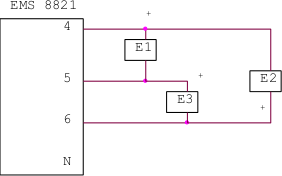
\includegraphics[width=.8\textwidth]{img/circuit_01}
  \caption{Single Phase Transformer Circuit for part one}
  \label{fig:circuit_01}
\end{figure}

\begin{figure}[H]
  \centering
  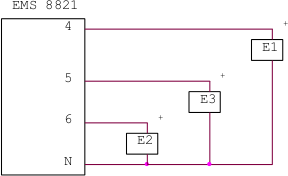
\includegraphics[width=.8\textwidth]{img/circuit_02}
  \caption{Single Phase Transformer Circuit for part two (open circuit test)}
  \label{fig:circuit_02}
\end{figure}

\begin{figure}[H]
  \centering
  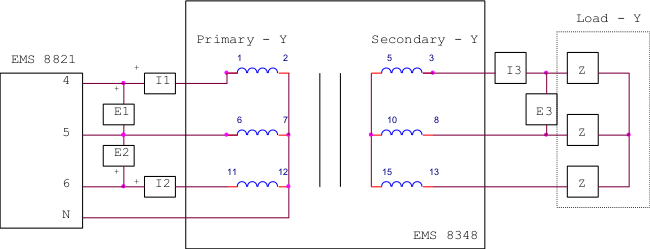
\includegraphics[width=.8\textwidth]{img/circuit_03}
  \caption{Single Phase Transformer Circuit for part two (short circuit test)}
  \label{fig:circuit_03}
\end{figure}

\end{document}
